\section{Licence plates}

Except for period plates, a vehicle must carry the plate format that matches the
date it was registered in Portugal. A newer format may be used, but an older one
may not, and doing so can be fined by the authorities.

\begin{figure}[htbp]
  \centering
  \begin{tabular}{@{}c c@{}}
    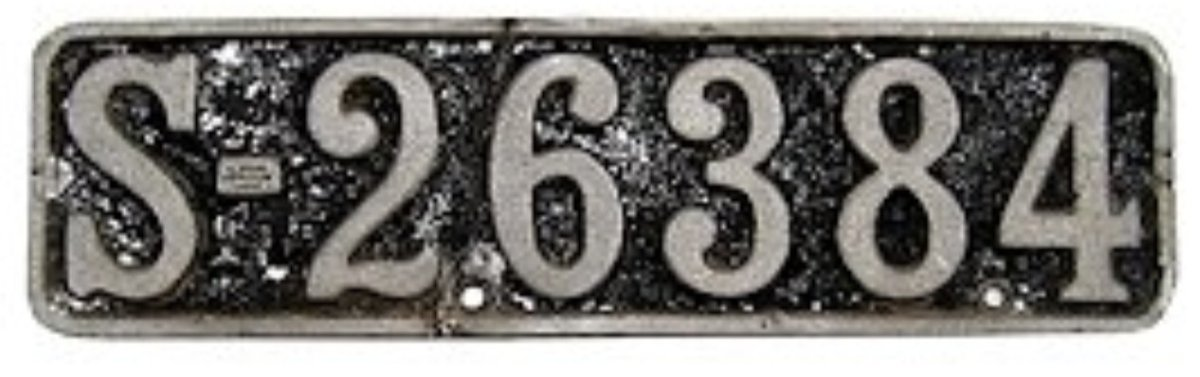
\includegraphics[height=1.3cm]{fmt-1911} & 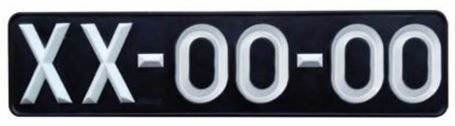
\includegraphics[height=1.3cm]{fmt-1937} \\
    \small 1911 to 31/12/1936 & \small 1/1/1937 to 31/12/1991 \\[0.6em]
    
\includegraphics[height=1.3cm]{fmt-1992} & 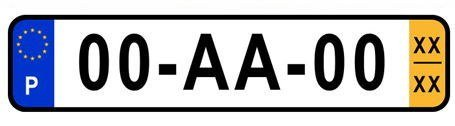
\includegraphics[height=1.3cm]{fmt-2005} \\
    \small 1/1/1992 to 31/12/1997 & \small 1/1/1998 to 2/3/2020 \\[0.6em]
    \multicolumn{2}{c}{
\includegraphics[height=1.3cm]{fmt-2020}} \\
    \multicolumn{2}{c}{\small From 3/3/2020}
  \end{tabular}
  \caption{The five plate formats and the period in which each look was issued. The 2023 edition gave 31/12/2019 and 1/1/2020. Decree-Law 2/2020 ties the
new plate design to the start of the new number format, and the first plate,
\plate{AA 01 AA}, was issued on 3 March 2020 (IMT).}
\end{figure}

Current plates follow the European model: a white reflective background with
black characters. On the left is the blue “euroband” with the national
identifier: \plate{P}.

Until the latest change, a yellow band on the right showed the month and year of
the vehicle's first registration (a car from June 1997, for example, would show
\plate{97/06}).

A car registered before 1 January 1998 may instead use the model in force when it
was registered:
\begin{itemize}
  \item black plates with white characters for cars registered up to
        31 December 1991;
  \item white plates with the blue euroband but no yellow band for cars
        registered between 1 January 1992 and 31 December 1997.
\end{itemize}

Old vehicles of museum interest may carry a plate of the model in force when they
entered service. Cars carry two plates, one at the front and one at the back
(Decree-Law 54/2005, art.~7; see section~\ref{sec:legislacao}).

\needspace{14\baselineskip}
\gen{series}
